\documentclass[runningheads]{llncs}
\usepackage[utf8]{inputenc}
\usepackage[T1]{fontenc}
%%\usepackage[
 %   top=2.5cm,
 %   bottom=2.5cm,
 %   left=3cm,
 %   right=3cm
%]{geometry}
\usepackage[french]{babel}
\usepackage{graphicx} % Required for inserting images
\usepackage{hyperref}
\usepackage{url}
\usepackage{amsfonts,amsmath,amssymb}
\usepackage{booktabs}
\usepackage{tabularx}
\usepackage{array}
\usepackage{xltabular}
\usepackage{xcolor}
\usepackage[authoryear,round]{natbib}




\title{Détection de deepfakes générés par des modèles de diffusion}
\author{Axcel Mugisha \and Victoria Pedoussat}
\authorrunning{A. Mugisha et V. Pedoussat}

\institute{
IMT \\
\email{\{axcel.mugisha,victoria.pedoussat\}@utoulouse.fr}
}

\date{May 2026}

\begin{document}

\maketitle
\begin{abstract}
    
\end{abstract}
\section*{CECI EST UN BROUILLON}

\section{Context}
Les progrès récents des modèles génératifs ont profondément transformé la création d’images numériques. Les premiers travaux de synthèse réaliste reposaient largement sur les GANs  (Generative Adversarial Networks) \citep{goodfellow2020generative} capables de produire des visages, objets ou scènes visuellement crédibles. Depuis 2021-2022, les modèles de diffusion \citep{NEURIPS2020_4c5bcfec}et les Latent Diffusion Models \citep{rombach2022highresolutionimagesynthesislatent}se sont imposés comme des architectures dominantes pour la génération text-to-image et image-to-image. Des systèmes tels que Stable Diffusion, Midjourney, DALL·E, GLIDE ou ADM produisent désormais des images réalistes à grande échelle, souvent difficiles à distinguer à l’œil nu d’images capturées par caméra \citep{nichol2022glidephotorealisticimagegeneration,dhariwal2021diffusionmodelsbeatgans}. Cette évolution soulève des enjeux majeurs en désinformation, preuve numérique, propriété intellectuelle et sécurité des systèmes multimédias. Les benchmarks récents comme GenImage \citep{zhu2023genimage} ont été construits précisément pour évaluer cette nouvelle génération de détecteurs sur des images issues à la fois de GANs et de modèles de diffusion.

La détection de deepfakes est devenue un problème central parce que la qualité des générateurs augmente très vite \citep{mirsky2021creation,rossler2019faceforensics}. Les anciennes méthodes détectaient souvent des défauts visibles : contours flous, yeux incohérents, artefacts de compression, mauvaise fusion du visage \citep{li2018ictu,li2019warping,rossler2019faceforensics,li2020facexray,afchar2018mesonet} . Mais les modèles modernes notamment les modèles de diffusion, les modèles vidéo génératifs et les modèles audio-visuels produisent des contenus beaucoup plus réalistes, ce qui rend la détection plus difficile.

Formellement, les détecteurs cherchent à, apprendre une fonction de décision
$$
    f(x)\to \{\text{réel,généré}\}
$$
où $x$ désigne une image ou une vidéo d’entrée. Cependant, le véritable défi n’est pas seulement d’obtenir une bonne performance sur un dataset donné mais aussi la généralisation : un détecteur entraîné sur les images d’un générateur donné doit idéalement reconnaître des images produites par des générateurs inconnus. Les travaux récents montrent que les détecteurs entraînés de manière supervisée sur un générateur peuvent obtenir de très bons résultats intra-dataset, mais perdre fortement en performance dès que les images proviennent d’un autre modèle ou subissent des transformations réalistes telles que compression JPEG, recadrage, flou ou redimensionnement\citep{ojha2024universalfakeimagedetectors}.


\section{Méthodes par reconstruction générative}

L’intuition centrale est la suivante : une image générée par un modèle de diffusion peut être plus proche de la distribution apprise par un autre modèle de diffusion ou par un autoencodeur latent. Elle peut donc être reconstruite différemment d’une image naturelle capturée par caméra. Les images réelles contiennent souvent des détails physiques, du bruit capteur, des textures naturelles ou des microstructures que le modèle génératif ne reconstruit pas exactement.


Au lieu d’entraîner uniquement un classifieur discriminatif qui apprend directement à séparer des images réelles et générées, on utilise un modèle génératif pré-entraîné pour reconstruire l’image suspecte, puis on analyse l’erreur entre l’image originale et sa reconstruction.

 

 \subsection{DIRE: Diffusion Reconstruction Error}
 La méthode DIRE \citep{wang2023dirediffusiongeneratedimagedetection} repose sur l’utilisation d’un modèle de diffusion pré-entraîné pour reconstruire une image. Pour comprendre cette idée, il faut d’abord rappeler brièvement le fonctionnement d’un modèle de diffusion.

Un modèle de diffusion part d’une image propre $x_0$, puis lui ajoute progressivement du bruit au cours d’un processus appelé processus forward. À une étape $t$, on obtient une version bruitée de l’image, notée $x_t$:
 
 $$
    x_t=\sqrt{\alpha_t}x_0+\sqrt{1-\alpha_t}\varepsilon
 $$
 où $\varepsilon$ est un bruit gaussien, $\varepsilon \sim \mathcal{N}(0,I)$ et $\alpha_t$ et $1-\alpha_t$ sont des coefficients qui contrôlent, respectivement, la quantité d'information conservée depuis l'image et la quantité de bruit ajoutée.

 Quand $t$ augmente, l’image $x_t$ devient de plus en plus bruitée. Le modèle de diffusion apprend ensuite le processus inverse : à partir de $x_t$ , il cherche à retrouver une image moins bruitée, jusqu’à reconstruire une image propre.
 Dans DIRE, on utilise cette capacité de reconstruction pour tester une image suspecte. Soit une image d’entrée $x$. On la considère comme une image initiale $x_0$, puis on lui applique une étape de bruitage

  $$
    x_t=\sqrt{\alpha_t}x_+\sqrt{1-\alpha_t}\varepsilon
 $$
 Ensuite, le modèle de diffusion tente de reconstruire l’image et on obtient une reconstruction
 $$
    \hat{x}=R_{diff}(x)
 $$
 où $R_{diff}$ désigne la reconstruction produite par le modèle de diffusion.

On calcule alors l’erreur DIRE :
$$
    E_{DIRE}(x)=|x - \hat{x}|
$$
Cette quantité est une carte d’erreur, de même taille que l’image Si cette carte a des valeurs faibles  ou présente une structure particulière, cela peut indiquer que l’image est proche de la distribution apprise par le modèle de diffusion. Si elle a des valeurs élevées ou localisées dans certaines zones spécifiques, cela peut révéler des différences entre image naturelle et image générée

Dans un détecteur complet, on peut ensuite apprendre un classifieur
$$
    f(E_{DIRE}(x))\to \{0,1\}
$$
 

\begin{figure}[htbp]
    \centering
    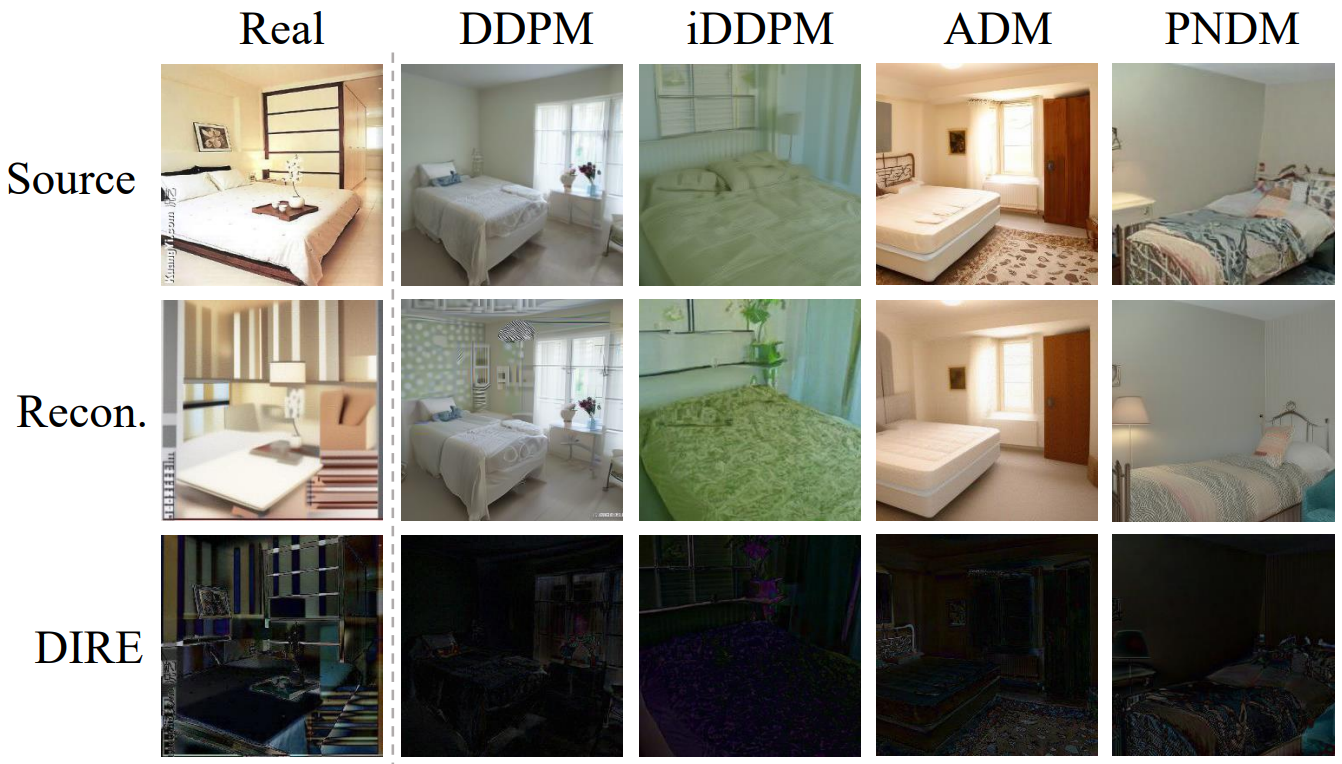
\includegraphics[width=0.8\textwidth]{Dire_teaser.png}
        \caption{\citep{wang2023dirediffusiongeneratedimagedetection}Representation DIRE d'une image réelle et des images générées par des models de diffusion: DDPM \citep{NEURIPS2020_4c5bcfec}, iDDPM \citep{nichol2021improveddenoisingdiffusionprobabilistic}, ADM\citep{dhariwal2021diffusionmodelsbeatgans}, et PNDM \citep{liu2022pseudonumericalmethodsdiffusion} respectivement. Les DIREs des images réelles tendent à avoir des grandes valeurs comparés aux images générées par les modèles diffusion.}
    \label{fig:schema_diffusion}
\end{figure}

\subsection{SeDID : erreur étape par étape dans le processus de diffusion}

Contrairement à des approches comme DIRE, qui comparent principalement une image d’entrée à sa reconstruction finale, SeDID\citep{ma2023exposingfakeeffectivediffusiongenerated} cherche à exploiter les erreurs intermédiaires produites au cours du processus de diffusion. SeDID définit d’abord une estimation de l’image propre:
$$
    f_\theta(x,t)=\frac{x-\sqrt{1-\bar{\alpha}_t}\varepsilon_\theta(x,t)}{\sqrt{\bar{\alpha}_t}}
$$
Dans cette expression, $\bar{\alpha}_t$ représente le coefficient cumulatif de conservation du signal au temps t. La fonction $f_\theta(x,t)$ permet donc d’estimer l’image initiale à partir d’un échantillon bruité.

A partir de cette estimation, SeDID introduit deux fonctions déterministes: La première est une fonction de débruitage, notée $\psi_\theta$ qui permet de passer d’un timestep $t$ vers un timestep moins bruité $t-\delta$:

$$
    \psi_\theta(x,t,\delta)=\sqrt{\bar{\alpha}_{t-\delta}}f_\theta(x,t)+\sqrt{1-\bar{\alpha}_{t-\delta}}\varepsilon_\theta(x,t)
$$
La seconde est une fonction reverse, notée $\phi_\theta$, qui réalise l’opération inverse, c’est-à-dire le passage de $t$ vers un timestep plus bruité $t+\delta$:


Le principe de SeDID consiste alors à prendre un échantillon intermédiaire 
$\tilde{x}_t$, à lui appliquer une étape reverse avec $\phi_\theta$, puis à revenir vers le timestep initial avec $\psi_\theta$. Si l’image est cohérente avec le modèle de diffusion, cet aller-retour doit reconstruire fidèlement l’échantillon intermédiaire. L’erreur utilisée par SeDID est donc définie par

$$
        E_{t,\delta}=\left\|\psi_\theta\left(\phi_\theta(\tilde{x}_t,t,\delta),t,\delta\right)-\tilde{x}_t\right\|^2
$$
Cette erreur mesure l’écart entre l’échantillon intermédiaire initial $\tilde{x}_t$ et l’échantillon obtenu après une opération reverse suivie d’une opération de débruitage.

Les auteurs introduisent ensuite un timestep spécifique, noté $T_{SE}$, qui correspond au moment où l’erreur stepwise est calculée. Le score de détection devient alors
$$
  E_{T_{SE},\delta}=\left\|\psi_\theta\left(\phi_\theta(\tilde{x}_{T_{SE}},T_{SE},\delta),T_{SE},\delta\right)-\tilde{x}_{T_{SE}}\right\|^2
$$

Deux variantes de SeDID sont proposées. La première, appelée $SeDID_{Stat}$, utilise directement cette erreur comme score statistique. La règle de décision peut être formulée ainsi
$$
    g(x)=\mathbf{1}\left[E_{T_{SE},\delta} < h\right]
$$
La seconde variante, appelée $SeDID_{NNs}$, utilise un réseau de neurones, par exemple ResNet, entraîné à partir des profils intermédiaires générés par les fonctions $\phi_\theta$ et $\psi_\theta$. Cette version ne se limite donc pas à un seuil sur une erreur scalaire : elle apprend directement des motifs discriminants à partir des états intermédiaires du processus de diffusion.

L’intérêt principal de SeDID est d’exploiter la dynamique interne du processus de diffusion plutôt qu’une simple erreur de reconstruction finale. Cette approche permet de capturer des différences subtiles entre images réelles et images générées. Toutefois, ses performances dépendent fortement du choix du timestep $T_{SE}$, du pas $\delta$ et du modèle de diffusion utilisé pour calculer les erreurs.
\begin{figure}[htbp]
    \centering
    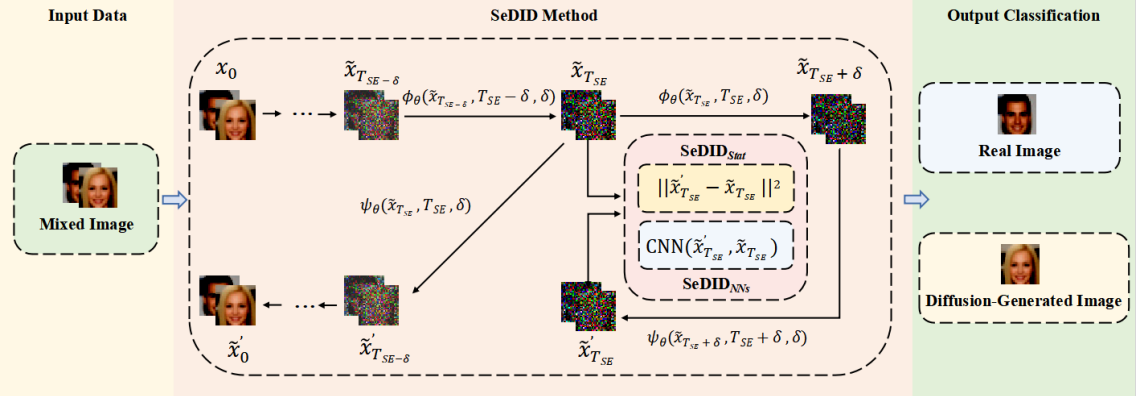
\includegraphics[width=1\linewidth]{SeDID.png}
    \caption{Pipeline de la méthode SeDID. À partir d’un ensemble d’images réelles et synthétiques, SeDID extrait un profil de bruit permettant de caractériser les images générées par diffusion. La méthode se divise ensuite en deux branches : une approche statistique, $\text{SeDID}{\text{Stat}}$, basée sur l’analyse des erreurs, et une approche par réseau de neurones, $\text{SeDID}{\text{NNs}}$, utilisant un ResNet entraîné par rétropropagation}
    \label{fig:placeholder}
\end{figure}

\subsection{AEROBLADE : reconstruction par autoencodeur latent}
AEROBLADE\citep{ricker2024aerobladetrainingfreedetectionlatent} se concentre sur les Latent Diffusion Models, comme Stable Diffusion. Dans ces modèles, l’image n’est pas directement traitée dans l’espace pixel pendant tout le processus de diffusion. Elle est d’abord projetée dans un espace latent plus compact.

On construit alors deux fonctions $\mathcal{E}(\cdot)$ l'encodeur et le décodeur $\mathcal{D}(\cdot)$. Donc pour une image $x$, l'encodeur produit un latent :
$$
     z=\mathcal{E}(x)
$$
puis le décodeur reconstruit une image à partir de ce latent :
$$
    \hat{x}=\mathcal{D}(z)
$$
 L'erreur produit par l'AEROBLADE peut donc s'écrire :
 $$
    E_{AE}(x)=|x-\mathcal{D}(\mathcal{E}(x))|
 $$
Après, on entraîne un classifieur sur cette erreur.

\begin{figure}[htbp]
    \centering
    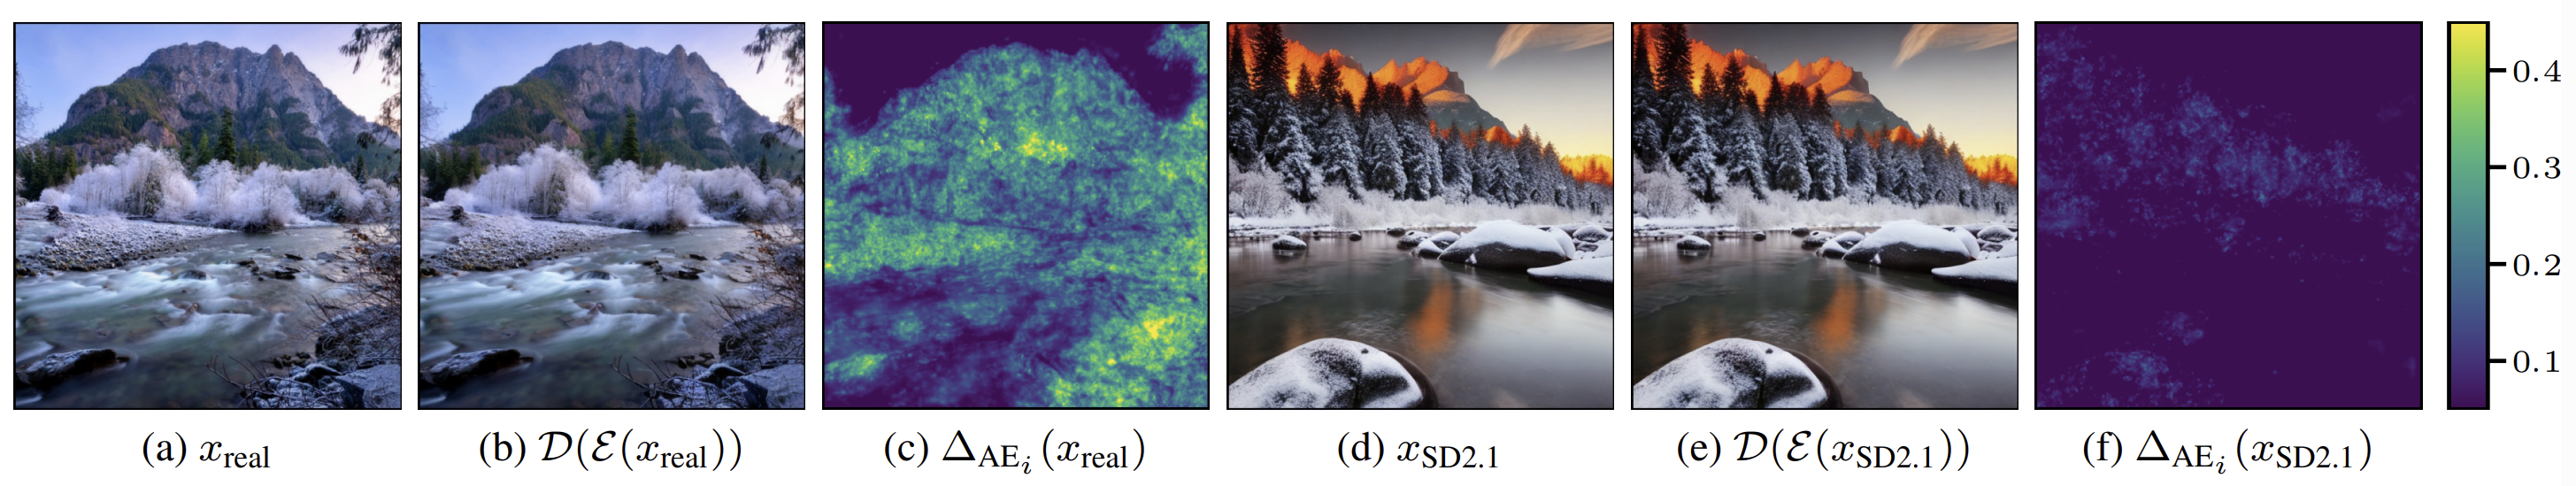
\includegraphics[width=1
    \linewidth]{AEROBLADE.png}
    \caption{\cite{ricker2024aerobladetrainingfreedetectionlatent}Exemple illustrant l'idée derrière AEROBLADE . (a) montre une image réelle et (d) illustre une image générée par Stable Diffusion 2.1 \cite{rombach2022highresolutionimagesynthesislatent}. (b) et (e) sont des reconstructions obtenues  en passant les images d'origine dans AEROBLADE de Stable DIffusion 2. (c) et (f) montrent les erreurs entre les images originales et leurs reconstructions mesuré en utilisant la distance LPIPS\citep{zhang2018unreasonableeffectivenessdeepfeatures}. L'erreur de reconstruction est significativement plus faible pour l' image générés $x_{SD2.1}$ que celle de l'image réelle $x_{real}$.}
    \label{fig:aeroblade}
\end{figure}
\subsection{LaRE² : erreur de reconstruction dans l’espace latent}

La méthode LaRE² \citep{10656812} pousse plus loin l’idée de reconstruction en travaillant non pas seulement dans l’espace image, mais dans l’espace latent. On commence par encoder l’image $z=\mathcal{E}(x)$ où $\mathcal{E}$ est l'encodeur VAE\citep{Kingma_2019}. Ensuite 
, on applique une perturbation de type diffusion dans l’espace latent. On note $z_t$ le latent bruité à l’étape t. De manière analogue au cas image, on peut écrire :
$$
    z_t=\sqrt{\alpha_t}z+\sqrt{1-\alpha_t}\varepsilon
$$
Le U-Net du modèle de diffusion reçoit généralement $z_t$, le temps $t$, et éventuellement une condition textuelle $c$ par exemple un embedding textuel dans le cas où le modèle de diffusion est un modèle texte-to-image. Il prédit le bruit ajouté:
$$
 \hat{\varepsilon}_\theta=\varepsilon_\theta(z_t,t,c)
$$
où $\varepsilon_\theta$ designe le U-Net de diffusion, paramétré par $\theta$ et $\hat{\varepsilon}_\theta$ est le bruit prédit par le modèle.

À partir de cette prédiction du bruit, on peut estimer le latent original
$$
    \hat{z}=\dfrac{z_t-\sqrt{1-\alpha_t}\hat{\varepsilon}_\theta}{\sqrt{\alpha_t}}
$$

L’erreur de reconstruction latente, appelée LaRE, peut alors être définie par
$$
    E_{LaRE}(x)=|z-\hat{z}|
$$

La différence avec DIRE est donc importante : DIRE mesure l’erreur dans l’espace image, tandis que LaRE² mesure l’erreur dans l’espace latent. L’espace latent est plus compact, LaRE² est  donc plus rapide que DIRE.

LaRE² ne se contente pas de calculer un score global. La méthode combine l’erreur latente avec des caractéristiques visuelles extraites par un backbone. On note $F=B(x)$ où $B$ est un backbone visuel, par exemple ResNet\citep{he2015deepresiduallearningimage} et $F$ est la feature map extraite de l’image. Comme $F$ et la carte $LaRE$ peuvent avoir des des dimensions différentes , pour pouvoir les combiner il faut aligner leurs dimensions. Ceci peut se faire par pooling ou projection par convolution. Notons $A$ ctte opération d'alignement:
$$
    \tilde{E}_{LaRE}=A(E_{LaRE})
$$
Ensuite, on peut utiliser l’erreur LaRE pour guider les features visuelles
$$
    F_{refined}=G(F,\tilde{E}_{LaRE})
$$
où G st donc cette opération de raffinement. La classification peut donc s'écrire
$$
    \hat{y}=\sigma(W\cdot Pool(F_{refined})+b)
$$
où $W$ et $b$ sont respectivement la matrice des poids et le biais qui sont appris pendant l’entraînement du classifieur.
\begin{figure}[htbp]
    \centering
    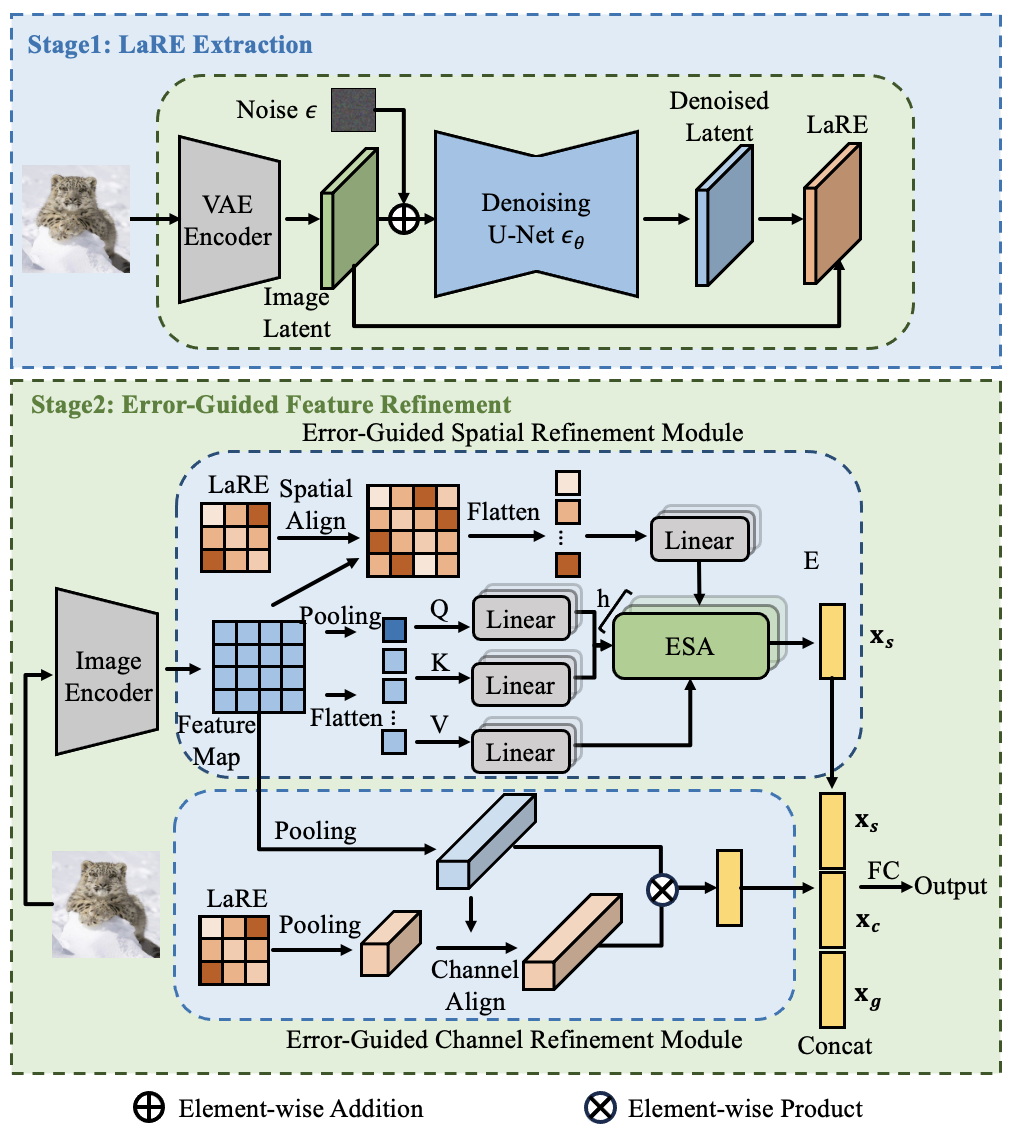
\includegraphics[width=0.8\linewidth]{Lare2.png}
    \caption{la méthode LaRE² extrait d’abord une carte d’erreur LaRE dans l’espace latent, puis utilise cette erreur pour dire au détecteur où regarder dans l’image et quels canaux de caractéristiques sont importants pour distinguer une image réelle d’une image générée}
    \label{fig:placeholder}
\end{figure}

\subsection{DRCT : reconstruction diffusion et apprentissage contrastif}
DRCT, pour Diffusion Reconstruction Contrastive Training\citep{chen2024drct}, combine l’idée de reconstruction diffusion avec l’apprentissage contrastif. L’idée générale de l’apprentissage contrastif est d’apprendre une représentation dans laquelle les exemples similaires sont proches et les exemples différents sont éloignés. On introduit une fonction d’encodage $g(\cdot)$ qui transforme une image $x$ en vecteur de représentation $u=g(x)$.

Dans DRCT, on peut considérer une image $x$ et sa version reconstruite par diffusion $\hat{x}$. On obtient alors deux représentations $u=g(x)$ et $\hat{u}=g(\hat{x})$. L'objectif est d'apprendre un espace de représentation où les relations entre images originales , images reconstruites , images réelles et images générées sont plus discriminantes. Une loss contrasive classique peut s'écrire sous la forme
$$
    \mathcal{L}_{\text{contr}}=y\,d(u_i,u_j)^2+(1-y)\max(0,m-d(u_i,u_j))^2
$$
où $d(u_i,u_j)$ mesure la distance entre deux représentations, $m$ est une marge, et $y$ indique si la paire doit être rapprochée ou éloignée.

Dans le contexte de la détection d’images générées, l’apprentissage contrastif permet d’apprendre des représentations plus robustes que la simple classification supervisée. Il peut aider le modèle à mieux distinguer les différences subtiles entre une image réelle, une image générée, et une image reconstruite par diffusion.

\begin{figure}[htbp]
    \centering
    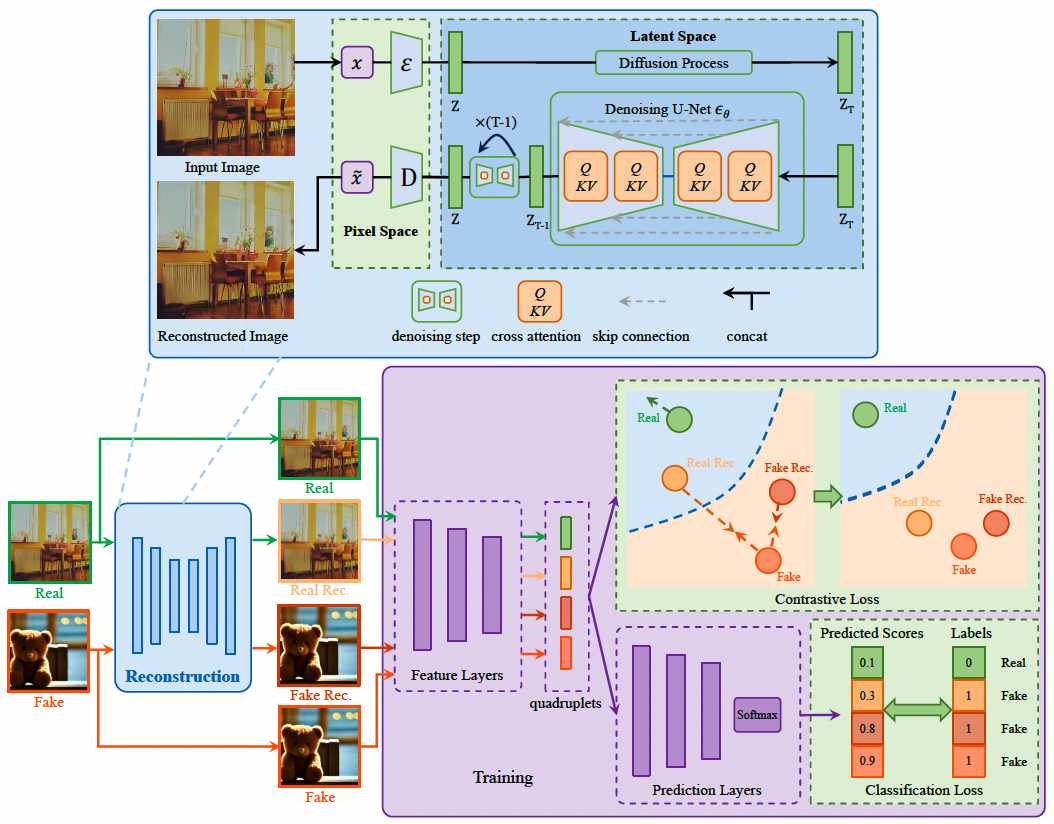
\includegraphics[width=1\linewidth]{DRCT.png}
    \caption{Le cadre DRCT se compose de deux étapes principales : une étape de reconstruction et une étape d’entraînement. Dans l’étape de reconstruction, une image d’entrée subit un processus de diffusion, puis elle est reconstruite à l’aide d’un réseau de débruitage. Dans l’étape d’entraînement, un classifieur binaire est entraîné sur des images réelles, des images générées, ainsi que sur leurs versions reconstruites. Une perte contrastive (contrastive loss) est utilisée pour guider l’apprentissage de caractéristiques discriminantes, tandis qu’une perte de classification est employée pour détecter les images générées.}
    \label{fig:placeholder}
\end{figure}







\subsection{DNF : Diffusion Noise Feature}
Contrairement aux approches fondées sur l'erreur de reconstruction, telles que DIRE\citep{Zhang_2025}, DNF ne compare pas directement l'image d'entrée $x$ à une reconstruction $\hat{x}$. La méthode applique plutôt un processus de diffusion inverse à l'image suspecte et collecte, à plusieurs timesteps, les bruits estimés par le modèle de diffusion.

On note $x_{t_k}$ l'état de l'image au timestep $t_k$, et $\varepsilon_\theta $ le réseau de diffusion pré-entraîné chargé d'estimer le bruit. Pour chaque timestep $t_k$, le bruit estimé est donné par 
$$
    \hat{\varepsilon}_{t_k}=\varepsilon_\theta(x_{t_k},t_k)
$$

La méthode collecte alors une séquence de bruits estimés 
$$
    \mathcal{N}(x)=\left\{\hat{\epsilon}_{t_1},\hat{\epsilon}_{t_2},\dots,\hat{\epsilon}_{t_K}\right\}
$$

Ces bruits sont ensuite fusionnés par une fonction $\mathcal{A}$ afin de produire la représentation appelée \text{Diffusion Noise Feature} 
$$
    \operatorname{DNF}(x)=\mathcal{A}\left(\hat{\epsilon}_{t_1},\hat{\epsilon}_{t_2},\dots,\hat{\epsilon}_{t_K}\right)
$$

Les auteurs étudient plusieurs stratégies de fusion. La première consiste à utiliser uniquement le premier bruit estimé :
$$
    \operatorname{DNF}_{\text{first}}(x)=\hat{\epsilon}_{t_1}
$$

La deuxième stratégie consiste à moyenner les bruits estimés sur les $K$ timesteps 
$$
    \operatorname{DNF}_{\text{mean}}(x)=\frac{1}{K}\sum_{k=1}^{K}\hat{\epsilon}_{t_k}
$$

Enfin, une stratégie apprenable consiste à empiler les bruits estimés puis à les fusionner à l'aide d'une convolution 3D 
$$
    \operatorname{DNF}_{\text{conv}}(x)
=\operatorname{Conv3D}
\left(\left[\hat{\epsilon}_{t_1},\hat{\epsilon}_{t_2},\dots,\hat{\epsilon}_{t_K}\right]\right)
$$

La représentation DNF obtenue est ensuite fournie à un classifieur, par exemple ResNet-50, afin de prédire si l'image est réelle ou générée 
$$
    \hat{y}=C_\omega\left(\operatorname{DNF}(x)\right)
$$
où $C_\omega$ désigne le classifieur entraîné et $\omega$ ses paramètres.

L'intérêt principal de DNF est que le processus de diffusion permet d'extraire une représentation plus discriminante que l'image brute. Les auteurs montrent que les bruits estimés peuvent révéler des différences subtiles entre images naturelles et images synthétiques, notamment dans les hautes fréquences. Ainsi, DNF transforme une image visuellement difficile à classifier en une représentation plus adaptée à la détection forensique. Toutefois, les performances de la méthode dépendent du modèle de diffusion utilisé pour extraire les bruits, du nombre de timesteps sélectionnés et de la stratégie de fusion adoptée.


\subsection{Your Diffusion Model is an Implicit Synthetic Image Detector}

Wang et Kalogeiton proposent une approche intitulée \textit{Your Diffusion Model is an Implicit Synthetic Image Detector}\citep{wang}, dans laquelle un modèle de diffusion pré-entraîné est utilisé comme un détecteur implicite d'images synthétiques . L'idée principale est qu'un modèle de diffusion, bien qu'il soit initialement entraîné pour générer ou débruiter des images, apprend une représentation riche de la distribution des images naturelles. Contrairement aux méthodes classiques qui entraînent directement un classifieur sur les pixels de l'image, cette approche analyse la manière dont un modèle de diffusion pré-entraîné réagit à une image lorsqu'elle est bruitée. L'image d'entrée $x$ est d'abord encodée dans l'espace latent du modèle de diffusion à l'aide de l'encodeur du VAE :
$$
    z = \mathcal{E}(x)
$$
où $\mathcal{E}$ désigne l'encodeur et $z$ la représentation latente de l'image. Ensuite, un bruit gaussien $\varepsilon \sim \mathcal{N}(0,I)$ est ajouté au latent à un timestep $t$, selon le schéma classique du processus de diffusion :
$$
    z_t =\sqrt{\bar{\alpha}_t}z+\sqrt{1-\bar{\alpha}_t}\varepsilon
$$

 Le latent bruité $z_t$ est ensuite donné au U-Net du modèle de diffusion, qui prédit le bruit contenu dans ce latent. Une particularité importante de cette méthode est qu'elle exploite à la fois la réponse conditionnelle et la réponse inconditionnelle du modèle de diffusion. En notant $c$ une condition textuelle et $\varnothing$ une condition vide, le bruit prédit sous condition est :
$$
    \hat{\varepsilon}_{\text{cond}}=\varepsilon_\theta(z_t,t,c)
$$
tandis que le bruit prédit sans condition est :
$$
    \hat{\varepsilon}_{\text{uncond}}=\varepsilon_\theta(z_t,t,\varnothing)
$$

Ces deux sorties traduisent deux manières différentes pour le modèle de diffusion d'interpréter l'image bruitée. La prédiction conditionnelle indique comment le modèle réagit lorsque l'image est analysée avec une information textuelle, tandis que la prédiction inconditionnelle révèle la réponse plus générale du modèle, sans guidage explicite.

La représentation forensique est alors construite à partir de ces différentes réponses internes. Une formulation possible consiste à combiner le bruit réel $\varepsilon$, le bruit prédit inconditionnel $\hat{\varepsilon}_{\text{uncond}}$, ainsi que l'erreur entre les deux 
$$
    F_t(x)=\operatorname{Concat}\left(\varepsilon^2,(\varepsilon-\hat{\varepsilon}_{\text{uncond}})^2,\hat{\varepsilon}_{\text{uncond}}^2\right)
$$


Lorsque plusieurs timesteps sont utilisés, on obtient une suite de représentations 
$$
    F_{t_1}(x), F_{t_2}(x), \dots, F_{t_K}(x)
$$
Ces représentations peuvent être empilées afin de former une représentation globale :
$$
    F(x)=\operatorname{Stack}\left(F_{t_1}(x),F_{t_2}(x),\dots,F_{t_K}(x)\right)
$$
La représentation $F(x)$ est ensuite donnée à un classifieur, par exemple un réseau de type ResNet, afin de prédire si l'image est réelle ou synthétique :
$$
\hat{y}
=
C_\omega(F(x)),
$$


L'intérêt de cette méthode est qu'elle transforme un modèle de diffusion en extracteur de caractéristiques forensiques. Le modèle de diffusion n'est pas entraîné explicitement pour la détection, mais ses réponses internes contiennent des informations discriminantes. C'est pourquoi les auteurs parlent de détecteur implicite : la capacité de détection émerge de la manière dont le modèle de diffusion réagit aux images réelles et synthétiques.



\begin{figure}[htbp]
    \centering
    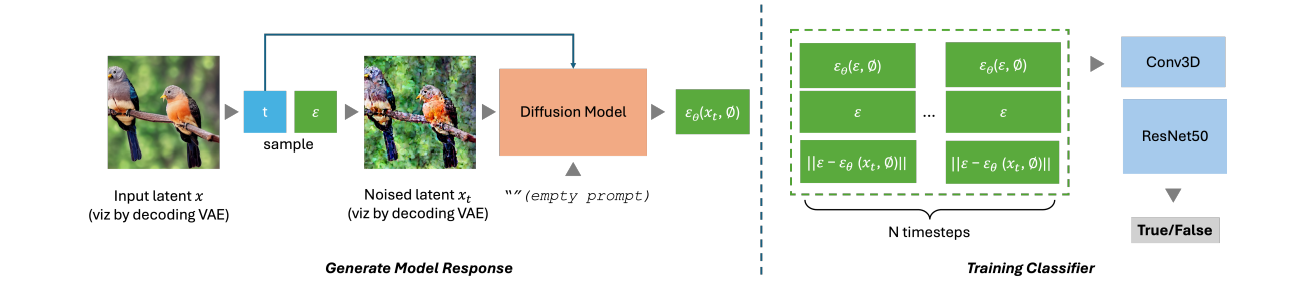
\includegraphics[width=1\linewidth]{yourmodel_detector.png}
    \label{fig:placeholder}
    \caption{
Le pipeline de la méthode comporte deux parties : un échantillonneur, à gauche, et un classifieur, à droite. Le rôle de l’échantillonneur est d’échantillonner et de collecter les réponses d’un modèle de diffusion pré-entraîné. Les données collectées sont ensuite fournies à un classifieur utilisant un backbone ResNet-50 afin de prédire si une image est réelle ou fausse.
}
\end{figure}


\subsection{DiffusionFake : Stable Diffusion comme guide d’apprentissage}

%\begin{figure}
%    \centering
%    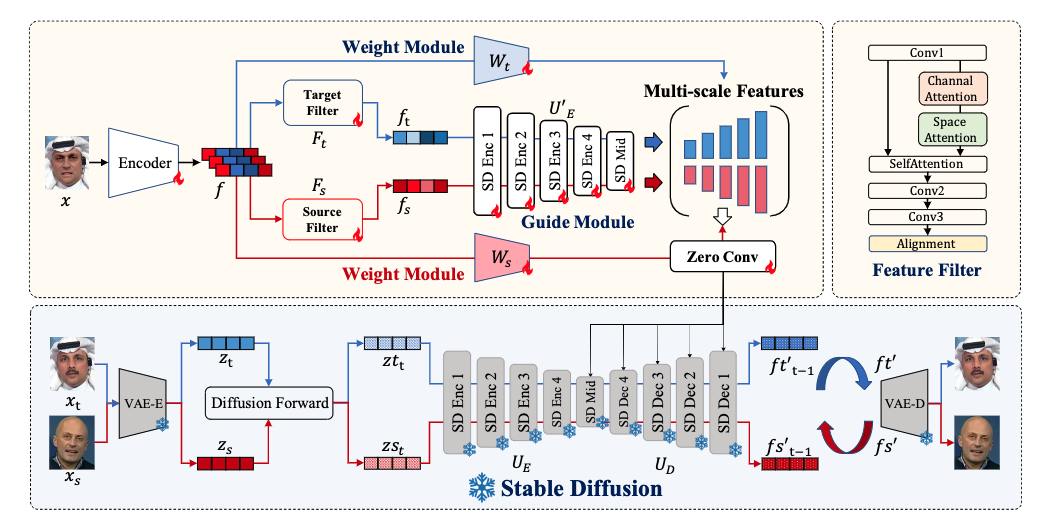
\includegraphics[width=0.8\linewidth]{difffake.png}
%    \caption{Caption}
%    \label{fig:placeholder}
%\end{figure}


DiffusionFake, proposé par Sun et al. \citep{sun2024diffusionfakeenhancinggeneralizationdeepfake}, est une méthode visant à améliorer la généralisation des détecteurs de deepfakes faciaux. Contrairement à des approches comme DIRE, SeDID, DNF ou LaRE\textsuperscript{2}, qui exploitent directement une erreur de reconstruction, un bruit prédit ou un signal intermédiaire du processus de diffusion, DiffusionFake utilise un modèle Stable Diffusion pré-entraîné et gelé comme guide pendant l'entraînement du détecteur. L'objectif est de forcer le détecteur à apprendre des représentations plus générales, liées aux identités source et cible présentes dans les images falsifiées.

L'idée principale repose sur le fait qu'une image deepfake, en particulier dans le cas du \textit{face swapping}, contient souvent un mélange d'informations provenant de deux identités. On note $x_s$ l'image source, correspondant à l'identité injectée, et $x_t$ l'image cible, correspondant au visage ou au contexte dans lequel l'identité est insérée. Pour une image réelle, on peut considérer que l'identité est cohérente, c'est-à-dire que les informations source et cible coïncident.\\
Soit une image d'entrée :
$$
    x \in \mathbb{R}^{H \times W \times C}
$$
Le détecteur extrait d'abord une représentation visuelle de cette image à l'aide d'un encodeur $E_\theta$
$$
    F = E_\theta(x)
$$
où $F$ désigne la carte de caractéristiques extraite et $\theta$ les paramètres de l'encodeur. Dans un détecteur classique, cette représentation serait directement transmise à une tête de classification. DiffusionFake ajoute cependant des modules auxiliaires afin d'obliger $F$ à contenir des informations utiles sur les composantes source et cible de l'image.

La méthode introduit deux modules de filtrage, notés $\mathcal{F}_s$ et $\mathcal{F}_t$. Le premier extrait une représentation orientée source 
$$
    F_s = \mathcal{F}_s(F)
$$
tandis que le second extrait une représentation orientée cible 
$$
    F_t = \mathcal{F}_t(F)
$$
Ainsi, \(F_s\) est censée contenir les informations liées à l'identité source, tandis que \(F_t\) contient les informations liées à l'identité cible. Ces modules permettent de séparer, dans les caractéristiques du détecteur, les informations qui peuvent révéler le mélange d'identités propre aux deepfakes.

DiffusionFake ajoute ensuite un module de pondération afin d'estimer l'importance relative des informations source et cible. On note ces poids 
$$
    w_s \quad \text{et} \quad w_t
$$

Les représentations pondérées sont ensuite injectées dans un module de guidage associé à Stable Diffusion. On peut écrire de manière simplifiée 
$$
    G_s = \mathcal{G}(w_s F_s)
$$
$$
    G_t = \mathcal{G}(w_t F_t)
$$
où \(\mathcal{G}\) désigne le module de guidage.

Le coeur de DiffusionFake consiste à utiliser un Stable Diffusion pré-entraîné et gelé pour imposer une contrainte de reconstruction sur ces représentations. Les images source et cible sont encodées dans l'espace latent du VAE de Stable Diffusion :
$$
    z_s = \mathcal{E}_{\text{VAE}}(x_s)
$$
$$
    z_t = \mathcal{E}_{\text{VAE}}(x_t)
$$
où $\mathcal{E}_{\text{VAE}}$ désigne l'encodeur du VAE. Un bruit gaussien $\varepsilon \sim \mathcal{N}(0,I)$ est ensuite ajouté à ces latents à un timestep $k$. Pour la source, on obtient 
$$
    z_{s,k}=\sqrt{\bar{\alpha}_k}z_s+\sqrt{1-\bar{\alpha}_k}\varepsilon,
$$
et pour la cible 
$$
    z_{t,k}=\sqrt{\bar{\alpha}_k}z_t+\sqrt{1-\bar{\alpha}_k}\varepsilon.
$$
Le U-Net de Stable Diffusion, noté \(\epsilon_{\text{SD}}\), prédit alors le bruit ajouté, en étant guidé par les représentations source et cible :
$$
    \hat{\varepsilon}_s=\varepsilon_{\text{SD}}\left(z_{s,k}, k, G_s\right)
$$
$$
    \hat{\varepsilon}_t=\varepsilon_{\text{SD}}\left(z_{t,k}, k, G_t\right)
$$
Les pertes de reconstruction associées sont définies par :
$$
    \mathcal{L}_{\text{src}}=\left\|\varepsilon-\hat{\varepsilon}_s\right\|_2^2
$$
$$
    \mathcal{L}_{\text{tgt}}=\left\|\varepsilon-\hat{\varepsilon}_t\right\|_2^2
$$
Ces pertes obligent les représentations $F_s$ et $F_t$, produites par le détecteur, à contenir suffisamment d'information pour guider Stable Diffusion dans la reconstruction des composantes source et cible.

En parallèle, le détecteur apprend la tâche principale de classification réel/faux. À partir de la représentation $F$, une tête de classification $C_\omega$ produit 
$$
    \hat{y}=C_\omega(F)
$$


La perte totale de DiffusionFake combine alors la perte de classification et les pertes auxiliaires de reconstruction source et cible 
$$
    \mathcal{L}=\mathcal{L}_{\text{cls}}+\lambda_s \mathcal{L}_{\text{src}}+\lambda_t \mathcal{L}_{\text{tgt}}
$$
où $\lambda_s$ et $\lambda_t$ contrôlent l'importance des contraintes de reconstruction. Lorsque les modules de pondération sont également supervisés, on peut ajouter une perte supplémentaire 
$$
    \mathcal{L}=\mathcal{L}_{\text{cls}}+\lambda_s \mathcal{L}_{\text{src}}+\lambda_t \mathcal{L}_{\text{tgt}}+\lambda_w\left(\mathcal{L}_{w_s}+\mathcal{L}_{w_t}\right)
$$

L'intérêt principal de DiffusionFake est d'utiliser Stable Diffusion comme un professeur génératif gelé. Le modèle de diffusion n'est pas utilisé pour produire directement la décision réel/faux, mais pour imposer au détecteur d'apprendre des représentations plus riches, capables de séparer les informations source et cible. Cette stratégie vise à réduire le surapprentissage aux artefacts spécifiques d'un générateur ou d'un dataset.

\subsection{FIRE : Frequency-guided Reconstruction Error}
FIRE \citep{Chu_2025} combine la reconstruction générative et l’analyse fréquentielle.Les auteurs observent que les modèles de diffusion peuvent avoir du mal à reconstruire certaines informations fréquentielles des images réelles, notamment dans les fréquences intermédiaires. Cette difficulté peut devenir un indice pour distinguer images réelles et images générées par diffusion.

On part d’une image x. On utilise un modèle de reconstruction, souvent fondé sur un autoencodeur ou un modèle de diffusion, pour produire $\hat{x}=R(x)$.

Dans une méthode classique, on calculerait simplement
$$
    E(x)=|x-\hat{x}|
$$

FIRE ajoute une étape de décomposition fréquentielle. On introduit une transformation $\mathcal{F}(\cdot)$ qui peut représenter une transformée de Fourier, une transformée DCT, ou plus généralement une décomposition en bandes de fréquences.

L’erreur fréquentielle peut alors s’écrire
$$
    E_{freq}(x)=|\mathcal{F}(x)-\mathcal{F}(\hat{x})|
$$
On peut aussi séparer l'image en bande
$$
    x=x_{low}+x_{mid}+x_{high}
$$
et pour chaque bande $k$ , on a 
$$
    E_k(x)=|\mathcal{F}_k(x)-\mathcal{F}_k(\hat{x})|
$$
où $\mathcal{F}_k$ extrait la bande fréquentielle $k$.

La décision finale peut utiliser un classifieur 
$$
    \hat{y}=f(E_{freq}(x))
$$ 
ou combiner plusieurs erreurs 
$$
    \hat{y}=f(E_{pixel}(x),E_{low}(x),E_{mid}(x),E_{high}(x))
$$

FIRE est intéressant car il évite de considérer l’erreur de reconstruction comme un seul score global. Il demande plutôt : dans quelles fréquences l’erreur apparaît-elle ? Sa limite est qu’il ajoute plusieurs choix techniques : type de transformée, bandes fréquentielles, taille des filtres, stratégie de fusion et robustesse aux transformations comme JPEG ou redimensionnement.






\subsection{LATTE : Latent Trajectory Embedding}
LATTE \citep{vasilcoiu2025lattelatenttrajectoryembedding} part d'une critique des méthodes précédentes: beaucoup d'approches exploitent une seule erreur ou un seul timestep. Or, lr processus de diffusion est séquentiel, il propose donc de modéliser l'évolution des représentations latentes sur plusieurs étapes de débruitage.

On suppose que l’image $x$ est encodée dans un espace latent $z_0=\mathcal{E}(x)$. On ajoute une branche dans la quelle $x$ passe dans un encodeur visuel qui donne en sortie:$ F_{\text{global}}$ une représentation globale de toute l’image et $F_{\text{vis}}$ qui est une matrice des tokens locaux qui décrivent les différentes zones de l’image.

Ensuite,au lieu d'observer un seul latent bruité $z_t$, on considère une séquence $ z_T,z_{T-1},\dotsc,z_1,z_0$.

LATTE raffine  chaque latent  avec des features visuelles par cross-attention:
$$
    \tilde{z}_{t_k}=\operatorname{CrossAttn}(z_{t_k},F_{\text{vis}})
$$

La trajectoire est ensuite agrégée, par exemple par average pooling :

$$
    \Phi(x)= \operatorname{AVGPooling}(\tilde{z}_0,\dots,\tilde{z}_{T})
$$

Ensuite, cet embedding de trajectoire est concaténé avec un token global de l’image,
$$
    F_{\text{fused}}=G(F_{\text{global}},\Phi(x))
$$
et la décision est prise par le classifieur 
$$
    \hat{y}=\sigma(W\cdot F_{\text{fused}}+b)
$$

L’intuition de LATTE est forte : deux images peuvent avoir une erreur finale similaire, mais des trajectoires de débruitage différentes. Une image réelle peut être corrigée progressivement d’une certaine manière, tandis qu’une image générée peut suivre une trajectoire plus régulière ou plus compatible avec le modèle génératif. LATTE est donc plus riche qu’une méthode single-step mais sa limite principale est le coût de calcul. 

\begin{figure}[htbp]
    \centering
    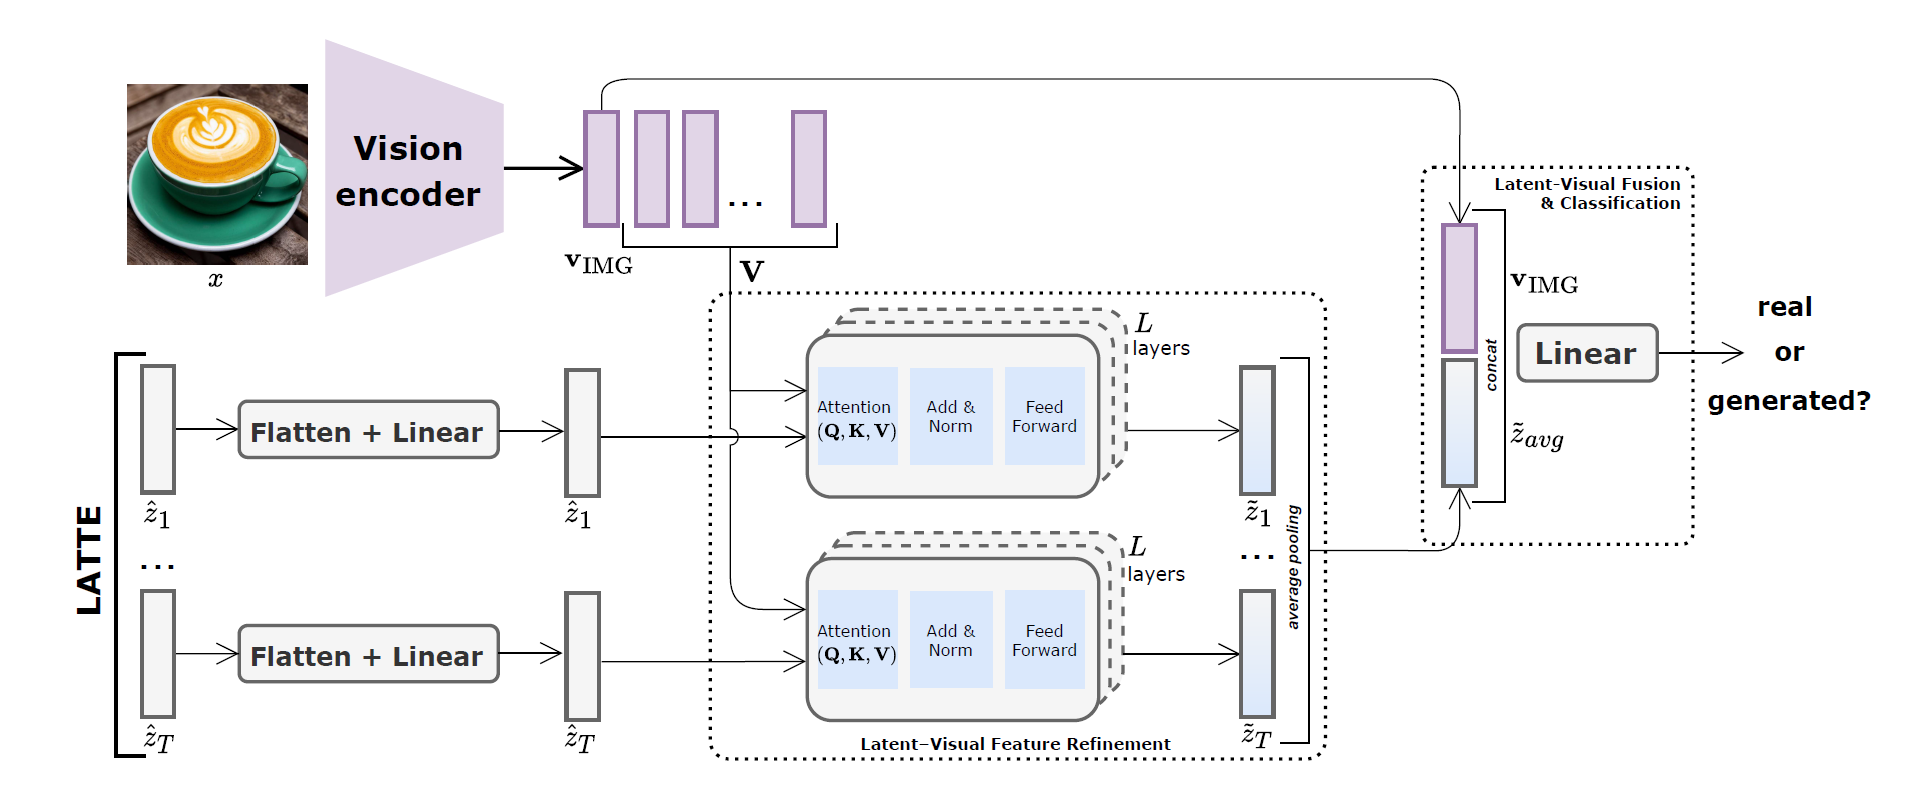
\includegraphics[width=0.8\linewidth]{latte_architecture.jpg}
    \caption{Vue d’ensemble de notre architecture proposée utilisant LATTE. Elle comprend deux étapes : (1)Fusion latent-visuel, où LATTE est fusionné avec la sémantique visuelle à travers une succession de L couches de cross-attention. (2)Classifieur latent-visuel, qui effectue une agrégation moyenne puis produit la prédiction finale.}
    \label{fig:placeholder}
\end{figure}

\subsection{ANL : Attention-guided Noise Learning}
La méthode ANL \citep{qi2026deepfake} est très récente et vise explicitement la généralisation des détecteurs de deepfakes aux modèles génératifs inconnus. Elle intègre un modèle de diffusion pré-entraîné dans le pipeline d’entraînement afin d’exploiter les caractéristiques du bruit de diffusion.

On part d'une image $x$, puis on crée une version bruitée $x_t$. Le modèle préentraîné , gelé, produit une estimation du bruit $\hat{\varepsilon}_\theta=\varepsilon_\theta(x_t,t)$. Le détecteur apprend lui aussi une représentation permetttant de prédire ce bruit. Notons cette prédiction
$$
    \tilde{\varepsilon}=h(F)
$$
où F est la feature map extraite par le détecteur et h est une tête de prédiction du bruit.

ANL ajoute ensuite une attention guidée par le bruit
$$
    A_{noise}=Attention(\tilde{\varepsilon},\hat{\varepsilon}_\theta)
$$
Cette attention est ensuite utilisée pour guider les features du détecteur
$$
    F_{ANL}=A_{noise}\odot F
$$
où $\odot$ désigne le produit élément par élément. La classification finale s'écrit donc
$$
    \hat{y}=\sigma(W\cdot Pool(F_{ANL})+b)
$$
et l'entraînement combine une losse de classification et une losse de bruit 
$$
    \mathcal{L}=\mathcal{L}_{cls}+\lambda\mathcal{L}_{noise}
$$
où $\lambda$ contrôle l’importance de la supervision par bruit.
\begin{figure}[htbp]
    \centering
    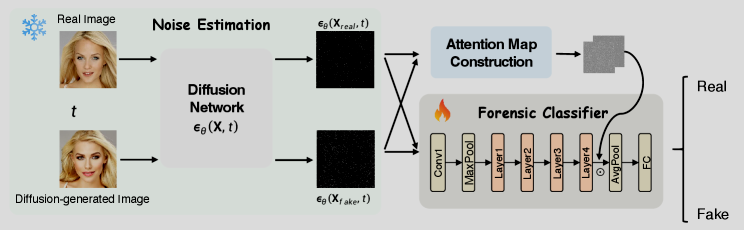
\includegraphics[width=1\linewidth]{ANL.png}
    \caption{Pipeline de l’apprentissage du bruit guidé par l’attention (ANL). ANL réalise l’estimation du bruit à l’aide du réseau d’estimation du bruit de diffusion, dans le processus inverse du DDPM \citep{NEURIPS2020_4c5bcfec}. Le bruit prédit est ensuite utilisé pour entraîner un classifieur forensique, par exemple ResNet \cite{he2015deepresiduallearningimage}, afin de distinguer les images réelles des images fausses, en le combinant avec la carte d’attention construite à partir du bruit prédit}
    \label{fig:placeholder}
\end{figure}

\newpage
\subsection{Tableau récapitulatif}


% Symboles
\newcommand{\cmark}{\checkmark}
\newcommand{\xmark}{\(\times\)}
\newcommand{\pmark}{\(\triangle\)} % partiel / indirect

\begin{table}[htbp]
\centering
\scriptsize
\renewcommand{\arraystretch}{1.15}
\begin{tabularx}{\textwidth}{
>{\raggedright\arraybackslash}p{2.8cm}
>{\centering\arraybackslash}p{1.4cm}
>{\centering\arraybackslash}p{1.7cm}
>{\centering\arraybackslash}p{1.3cm}
>{\centering\arraybackslash}p{1.4cm}
>{\centering\arraybackslash}p{1.4cm}
}
\toprule
\textbf{Méthode} 
& \textbf{Reconstr.} 
& \textbf{Bruit / U-Net} 
& \textbf{Latent} 
& \textbf{Multi-\(t\)}
& \textbf{Hybride} \\
\midrule

\textbf{DIRE} 
& \cmark 
& \pmark 
& \xmark 
& \pmark 
& \xmark \\

\textbf{SeDID} 
& \pmark 
& \cmark 
& \xmark 
& \cmark 
& \pmark \\

\textbf{DNF} 
& \xmark 
& \cmark 
& \pmark 
& \cmark 
& \pmark \\

\textbf{AEROBLADE} 
& \cmark 
& \xmark 
& \cmark 
& \xmark 
& \xmark \\

\textbf{LaRE\textsuperscript{2}} 
& \cmark 
& \cmark 
& \cmark 
& \pmark 
& \cmark \\

\textbf{DRCT} 
& \cmark 
& \pmark 
& \pmark 
& \pmark 
& \cmark \\

\textbf{Implicit Detector} 
& \xmark 
& \cmark 
& \cmark 
& \cmark 
& \pmark \\

\textbf{DiffusionFake} 
& \pmark 
& \cmark 
& \cmark 
& \pmark 
& \cmark \\

\textbf{FIRE} 
& \cmark 
& \pmark 
& \pmark 
& \pmark 
& \cmark \\

\textbf{LATTE} 
& \pmark 
& \cmark 
& \cmark 
& \cmark 
& \cmark \\

\textbf{ANL} 
& \xmark 
& \cmark 
& \pmark 
& \pmark 
& \cmark \\

\bottomrule
\end{tabularx}
\caption{Comparaison synthétique des méthodes exploitant les modèles de diffusion pour la détection de deepfakes. Le symbole \(\checkmark\) indique que la caractéristique est centrale dans la méthode, \(\times\) indique qu’elle n’est pas utilisée, et \(\triangle\) indique une utilisation partielle ou indirecte. La colonne \textit{Hybride} indique si la méthode combine un signal issu de la reconstruction ou du bruit de diffusion avec une autre technique, comme l’attention, l’analyse fréquentielle, l’apprentissage contrastif ou un classifieur dédié.}
\label{tab:comparison_diffusion_detection_methods}
\end{table}

%\textcolor{red}{TODO: faire une sous section pour les méthodes hybrides pour developper un peu }

\section{Bases de données de vidéos/photos générées par des modèles de diffusion}

Les premières bases de données dédiées à l'étude de détection de deepfakes étaient surtout générées par des GANs ou des autoencodeurs, comme FaceForensics++ \citep{rossler2019faceforensics} ou bien CelebDF \citep{li}, qui sont des datasets de vidéos deepfakes célèbres. L'évolution récente des modèles de diffusion produisant des deepfakes plus réalistes avec des rendus visuels plus cohérents rend nécessaire l'introduction de bases de données deepfakes exclusivement générés par les modèles de diffusion afin de pouvoir étudier leur détection.

\bigskip

La plupart des datasets de deepfakes contiennent à la fois des vidéos ou des images réelles et des vidéos ou images fake.

Actuellement, les datasets existants de deepfakes générés par modèles de diffusion contiennent davantage des images que des vidéos. Nous évoquerons donc également des datasets d'images, bien que nous nous concentrerons sur les datasets vidéos.

Les datasets existants peuvent être regroupés en trois catégories : les datasets de deepfakes faciaux, les datasets généralistes de vidéos générées par intelligence artificielle, et les bases de données issues de contenus réels collectés en ligne.

\subsection{DigiFakeAV}

Le dataset DigiFakeAV \citep{liu} constitue l’une des bases de données les plus pertinentes pour l’étude des deepfakes générés par modèles de diffusion. Il contient environ 60 000 vidéos; avec environ 10 000 vidéos réelles et 50 000 vidéos fakes. Les contenus sont générés à l’aide de plusieurs modèles de diffusion, comme Sonic \citep{ji} ou encore Hallo \citep{xu}.

Cette base de données présente plusieurs avantages : plusieurs modèles génératifs sont utilisés, en particulier plusieurs modèles de diffusion, il y a une diversité d’ethnie et de genre, et la qualité visuelle des contenus générés est élevée.

DigiFakeAV peut donc être particulièrement utile pour étudier les artefacts introduits par les modèles de diffusion.

\subsection{TalkingHeadBench}

TalkingHeadBench \citep{xiong} est un benchmark récent conçu pour évaluer la détection des deepfakes de type "têtes parlantes", qui utilise des générateurs avancés et récents. Il contient 2 994 vidéos fake de haute qualité issues de huit générateurs différents, dont certains modèles de diffusion comme Hallo \citep{xu2024} et AniPortrait \citep{wei}, ainsi que 2 312 vidéos réelles.

Ce dataset a fait l'objet d'un processus de sélection qui a permis de filtrer plus de 60\% des échantillons afin d'éliminer les vidéos présentant des artefacts trop visibles et évidents, ce qui représente un défi plus difficile à relever pour les détecteurs.

Ce dataset est particulièrement pertinent pour tester la capacité de généralisation des détecteurs face à des changements d'identité ou de modèles génératifs, révélant que les systèmes performants sur des jeux de données plus anciens (comme FaceForensics++ \citep{rossler2019faceforensics}) rencontrent des difficultés importantes lorsqu'ils sont testés sur TalkingHeadBench.

\subsection{MAVOS-DD}

Le benchmark MAVOS-DD \citep{croitoru} est une base de données multimodale dédiée à la détection de deepfakes audio-visuels. Il contient plus de 250 heures de vidéos réelles et fake (91h de vidéos réelles et 161h de fakes) générées à partir de plusieurs familles de modèles génératifs, incluant certains modèles de diffusion, comme Sonic \citep{ji}.

L’intérêt de MAVOS-DD réside dans son approche dite open-set; les modèles de détection sont évalués sur des types de deepfakes qui n’ont pas forcément été observés pendant la phase de training, permettant ainsi d’étudier leur capacité de généralisation face à de nouveaux générateurs.

Cependant, la génération des deepfakes n'ayant pas exclusivement été faite par des modèles de diffusion, l'utilisation de ce dataset entraînerait une certaine sélection.

\subsection{GenVidBench}

GenVidBench \citep{ni} est un benchmark orienté vers les vidéos générées par l'intelligence artificielle, principalement à partir de scénarios text-to-video et image-to-video. Cependant, GenVidBench couvre un ensemble plus large de contenus synthétiques, et pas seulement des contenus faciaux. Avec plus de 143 000 vidéos, c'est l'un des plus vastes benchmarks de contenu IA général (personnes, animaux, plantes...). Cependant, il y a seulement 9,5\% de vidéos avec des humains.

Le benchmark inclut des vidéos générées par différents modèles de diffusion récents tels que Stable Video Diffusion \citep{blattmann}, ou VideoCrafter2 \citep{chen2}. Il permet notamment d’étudier la cohérence temporelle, les artefacts inter-frame, les anomalies de mouvement et les signatures fréquentielles des vidéos générées.

GenVidBench utilise une approche "cross-source" et "cross-generator". Les sources de génération (prompts ou images) et les générateurs eux-mêmes diffèrent entre l'entraînement et le test pour éviter que le détecteur ne se base sur le contenu de la vidéo plutôt que sur les traces de manipulation artificielle.

Bien qu’il ne soit pas exclusivement dédié aux deepfakes faciaux, GenVidBench peut représenter un complément pour l’analyse des vidéos deepfakes.

\subsection{Political Deepfakes Incidents Database (PDID)}

La base de données Political Deepfakes Incidents Database (PDID) \citep{walker} se concentre sur de véritables incidents politiques de deepfakes et "cheapfakes". Les "cheapfakes" sont des contenus réels modifiés par des techniques simples comme des montages, qui ne sont pas générés par l'intelligence artificielle. 

Ce dataset regroupe des contenus du monde réel collectés depuis 2017, postés par exemple sur les réseaux sociaux, parmi lesquels figurent des personnalités politiques majeures ainsi que des évènements géopolitiques mondiaux.

Ce dataset contient des informations détaillées ajoutées par les chercheurs. Ils précisent par exemple dans quel but le deepfake a été généré (blague, truquage, etc.) et quels ont été ses effets réels. 

Cependant, les outils de génération des contenus de ce dataset ne sont pas précisés, mais son utilisation peut être intéressante pour tester les modèles de détection avec des deepfakes qui ont vraiment été utilisés à des fins malveillantes. Il constitue ainsi un outil pertinent pour analyser les tendances de la désinformation politique et évaluer l'efficacité des solutions de détection dans des scénarios de menaces concrètes. 

\subsection{Datasets d’images complémentaires}

En raison du nombre encore limité de datasets vidéos exclusivement générés par modèles de diffusion, plusieurs bases de données d’images peuvent également être utilisées. Ces datasets permettent d’étudier les signatures intrinsèques des modèles de diffusion, qui peuvent être retrouvées dans les vidéos.

Nous pouvons citer par exemple :
\begin{itemize}
    \item GenImage \citep{zhu2023genimage} : benchmark massif d'images générées par des GANs et des modèles de diffusion, contenant des deepfakes, des images d'animaux ou encore des paysages.
    \item DeepFakeFace \citep{song} : dataset de deepfakes de célébrités générés par diffusion, créé pour entraîner et tester des algorithmes de détection de deepfake.
    \item DiFF \citep{cheng} : base de données de plus de 500 000 visages fake générés par 13 modèles de diffusion. Les auteurs proposent également une méthode de détection basée sur les graphes de contours.
    \item DiffusionFace \citep{chen} : jeu de données de deepfakes générés par diffusion, regroupant 600 000 images de haute qualité générées par 11 modèles différents.
\end{itemize}



\newpage
\bibliographystyle{plainnat}
\bibliography{ref}
\end{document}


 